\chapter{Introduction}

We shall begin this thesis with a puzzle. Consider the lattice depicted in the leftmost diagram of Figure \ref{fig:simple_puzzle}. We refer to the elements of this lattice as \emph{cells}. Suppose we have the capacity to infect some cells (colored red) with a disease, and that this disease will, over a period of time, propagate through uninfected cells of the lattice. Let uninfected cells become infected if they are exposed to at least two infected neighboring cells in the vertical and/or horizontal directions. We say that the initial infection is \emph{lethal} if the entire lattice ultimately becomes infected. Here is the puzzle:

\begin{question}
\label{que:simple_puzzle}
What is the fewest number of infected cells necessary to spawn a lethal infection?
\end{question}

\begin{figure}[]
\centering
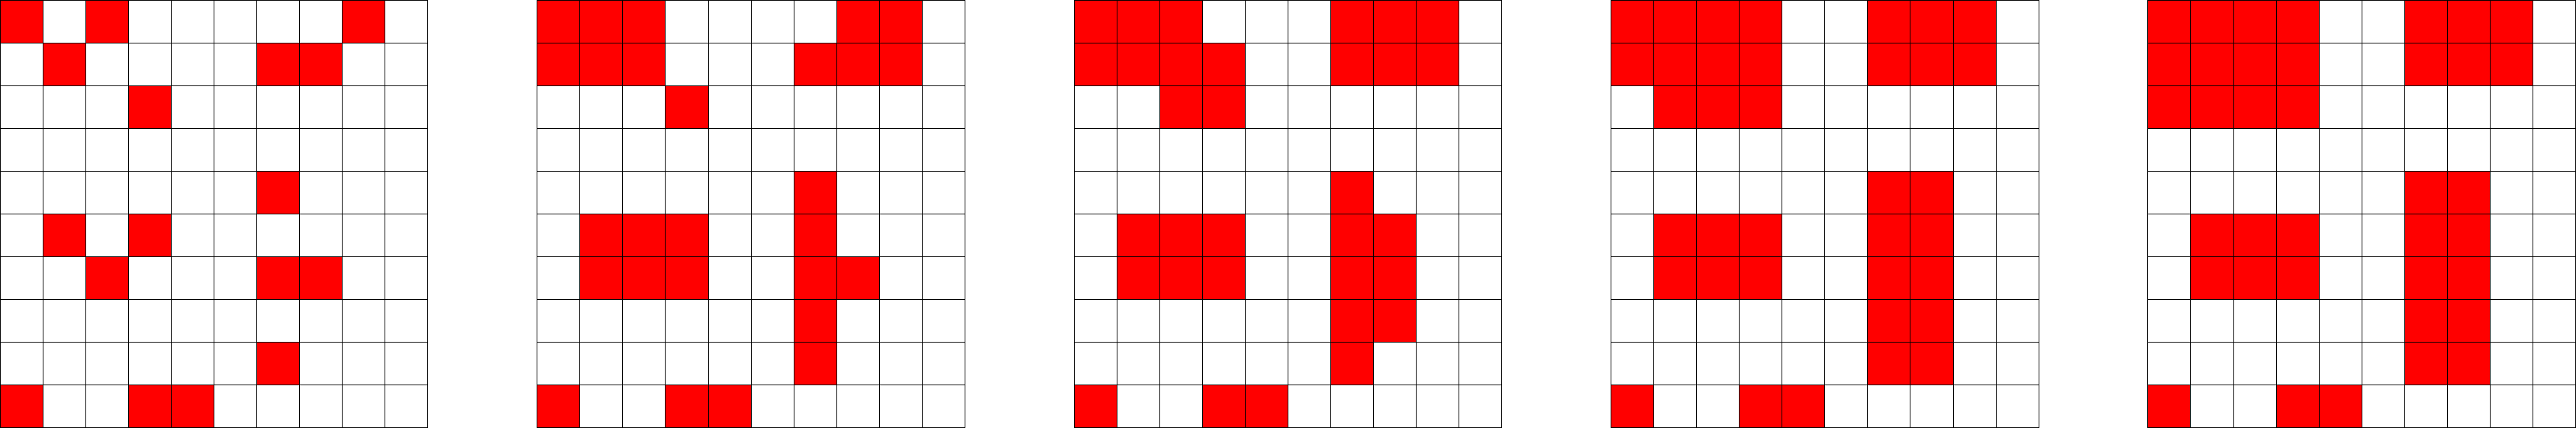
\includegraphics[width=\textwidth]{figures/1/simple_puzzle.pdf}
\caption{An arbitrary set of initially infected cells in the $10 \times 10$ lattice, and the stages of infection.}
\label{fig:simple_puzzle}
\end{figure} 

Before we present the solution,
%(which is particularly elegant and satisfying, and the reader is encouraged to play around with this problem on their own and get a feel for the behavior), 
let us take a moment to examine some properties of infectious sets and attempt to characterize what attributes might correspond to lethality. It should not take too long to observe that if an initial infection is in some way ``spread too thin," it will be unable to jump between infected areas, leading to gaps in infection, which we refer to as \emph{immune regions}. The perimeter of the lattice is particularly susceptible to this, as vertices there have fewer neighbors from whom they might be exposed. Heuristically, then, a lethal set must have the ability to effectively span the entire lattice, and must be particularly virulent along the perimeter. 

With this criteria in mind, we are able to make some educated guesses regarding the specific structure of sets that are likely to be lethal. In particular, we would like to consider the two starting infections illustrated in Figure \ref{fig:two_infections}. Notice that while Figure \ref{fig:two_infections} (\subref{fig:two_infections_b}) has far fewer perimeter infections, both (\subref{fig:two_infections_a}) and (\subref{fig:two_infections_b}) manage to form continuous bands of infected cells that appear to span the entire lattice after one step. Indeed, this holds with our notion of immune regions (or lack thereof), and we see that both infections will continue to propagate outwards from these bands until all cells become infected.

\begin{figure}[]
\centering
\begin{subfigure}{0.45\textwidth}
	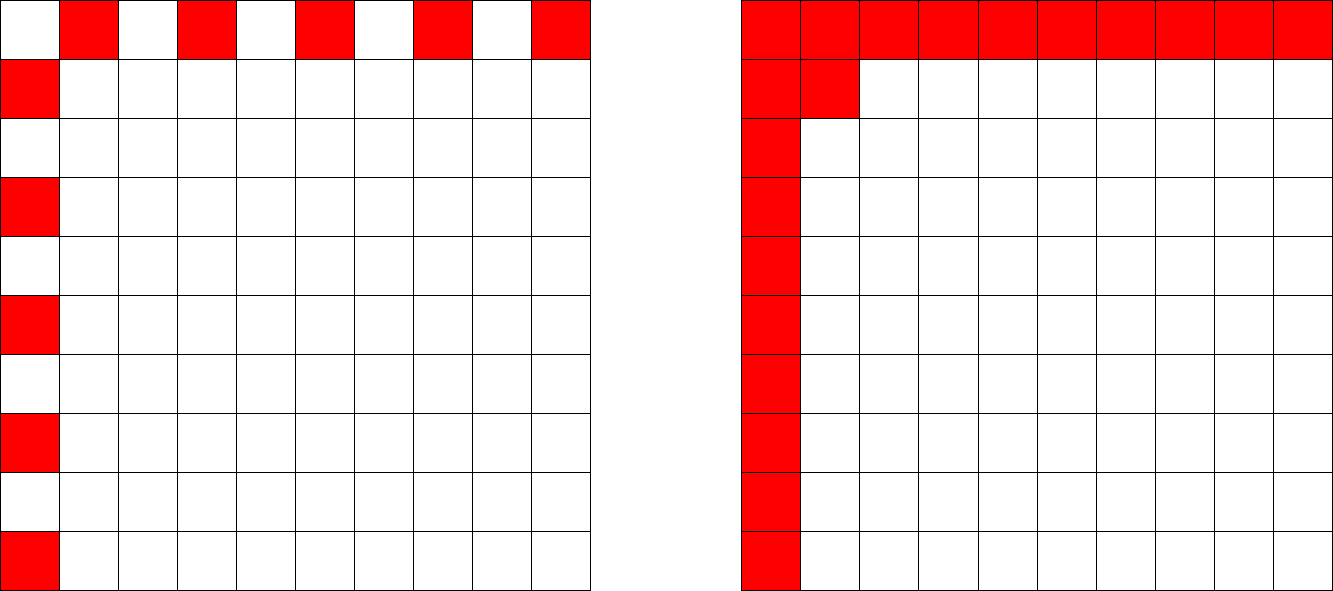
\includegraphics[width=\textwidth]{figures/1/two_infections_a.pdf}
	\caption{Perimeter construction.}
	\label{fig:two_infections_a}
\end{subfigure} \hfill%
\begin{subfigure}{0.45\textwidth}
	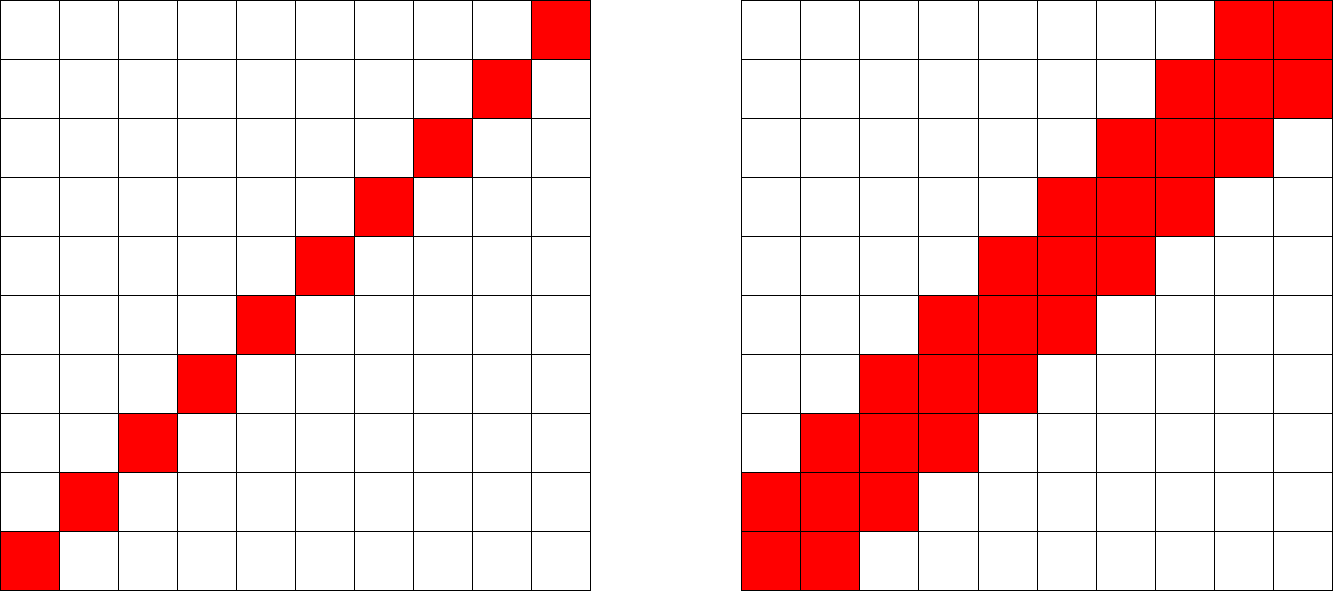
\includegraphics[width=\textwidth]{figures/1/two_infections_b.pdf}
	\caption{Diagonal construction.}
	\label{fig:two_infections_b}
\end{subfigure}
\caption{Two lethal sets and their resulting infections after one time-step.}
\label{fig:two_infections}
\end{figure} 

It is clear from Figure \ref{fig:two_infections} that we may obtain lethal sets on the $n \times n$ lattice of size $n$ by simply infecting the diagonal. What is less obvious is whether it is possible to improve upon this result. Perhaps the most natural first attempt at this is to remove an infection from one of the cells along the diagonal. However, this seems to form an immune region around the removed cell. After some experimentation, one begins to believe it impossible to simultaneously satisfy the heuristic that a starting infection must span the lattice, while also using fewer than $n$ initial infections. The question therefore becomes: how do we prove it?

Consider the cumulative perimeter of infected regions. For a given initial infection $A_0$, each cell in $A_0$ contributes at most $4$ to this perimeter, one for each of its sides. (This number may be lower, if two infected cells are adjacent. In such a case, one side of each cell lies within the infected region, and cannot contribute to the infection's perimeter.) Observe that for any uninfected cell to become infected, it must abut at least two infected cells. Upon infection, the edges abutting these cells no longer lie on the infection's perimeter; additionally, the remaining edges of this newly infected cell contribute at most $2$ to the perimeter of infection. All told, after infection, the resulting perimeter cannot increase. 

If we suppose that $A_0$ is a lethal set, then at some point in time, the entire grid will become infected. This infection will have a perimeter of $4n$. Since this perimeter cannot have increased, $A_0$ must have originally had a perimeter of at least $4n$. Since each cell in $A_0$ can contribute at most $4$ to this perimeter, it must be the case that $|A_0| \geq n$. Our diagonal construction shows that $|A_0| \leq n$, and so we are able to conclude that $n$ is best possible.

\section{Bootstrap Percolation}

%Before presenting a proof, let us take a moment to formally define the process described above and develop some useful notation. 
The study of such cellular infection spread in grids (and more generally in graphs) is known in the literature as \emph{bootstrap percolation}, and was introduced in the 1970s by Chalupa et al. \cite{chalupa:1979} as a simplified model for the behavior of ferromagnetic fields. In their original 1979 paper, the authors research the stable structure of probabilistically selected initial infections. While this differs from the problem posed in question \ref{que:simple_puzzle}, the rules for the spread of infection and its broad behavior remain the same. It is worth noting that a large portion of contemporary research on bootstrap problems is focused on questions of probabilistic nature; while these problems are certainly of merit and interesting, they do not fall within the scope of this thesis. Rather, we shall focus on those problems where we have specific control over the structure of the initial infections; in particular, we aim to determine the smallest lethal set on a variety of graph classes. 

We define the problem in concrete terms. Let $G$ be a graph and $A_0 \subseteq V(G)$ be a set of initially infected vertices. Iteratively, infect those vertices of $G$ with at least $r$ infected neighbors. For all $t > 0$, let $A_t$ be the set of infected vertices at time step $t$. We then have
$$A_t = A_{t-1} \cup \{v \in V(G) : |N_G(v) \cap A_{t-1}| \geq r\},$$
where $N_G(v)$ is the set of vertices adjacent to $v$ in $G$. We define the \emph{closure} of $A_0$ under $r$-neighbor bootstrap percolation to be $[A_0] = \bigcup_{t=0}^{\infty} A_t$. We say that $A_0$ \emph{percolates} or is \emph{lethal} if $[A_0] = V(G)$. We define the smallest percolating set on a graph $G$ under $r$-neighbor bootstrap percolation by the quantity $m(G,r)$. We note that under these rules, it is not possible for vertices to become uninfected.

There are a number of natural generalizations of the problem posed in Question \ref{que:simple_puzzle}. Of primary interest to the author are those obtained by varying the structure of $G$ and the value of $r$. Below, we outline some of the existing results for graphs that are the Cartesian product of paths and cycles, and $r \in \{0, 1, 2, 3\}$. These results are summarized in Table \ref{tab:known_bounds}.

\begin{table}[]
\centering
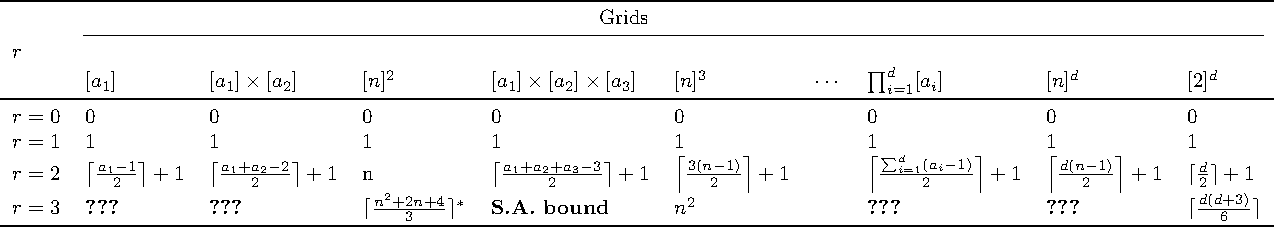
\includegraphics[width=\textwidth,origin=c]{tables/1/known_bounds.pdf}
\caption{A summary of known bootstrap percolation results for grids and the torus, $r \in \{0,1,2,3,d\}$.}
\label{tab:known_bounds}
\end{table} 

% r=0 and r=1
\subsection{$m(G,0)$ and $m(G,1)$} 

In the case where $r \in \{0,1\}$, the structure of $G$ is less important. We have the following results:

\begin{thm}
For all undirected, simple $G$, $m(G,0) = 0$.
\end{thm}

\begin{proof}
As cells need not be adjacent to infections to become infected, $A_1 = V(G)$, and so $A_0 = \emptyset$ is lethal.
\end{proof}

\begin{thm}
Let $G$ be an undirected, simple graph with $c$ components. Then $m(G, 1) = c$.
\end{thm}

\begin{proof}
Let $A_0$ be lethal. As infections spread along all edges, it is both necessary and sufficient for each connected component of $G$ to contain exactly one vertex of $A_0$. Therefore, $|A_0| = m(G,1) = c$.
\end{proof}

% r=2
\subsection{$m(G,2)$} 

We consider three classes of generalizations: the Cartesian product of paths, the Cartesian product of cycles, and the Cartesian product of both. 

\subsubsection{Grid: $P_a \square P_b$}

Recall from the discussion of Question \ref{que:simple_puzzle} that $m(P_n \square P_n,2) = n$, where the tight construction for the lower bound is given by a diagonal infection expanding laterally outwards. We generalize this result to all rectangular grids.

\begin{thm}
For $a, b \geq 1$,
$$m(P_a \square P_b,2) = \ceil*{\frac{a+b-2}{2}}+1.$$
\end{thm}

\begin{proof}
We apply the perimeter argument to obtain a lower bound, and then show that this lower bound is tight by generalizing the diagonal construction presented above.
\end{proof}

\subsubsection{Grid: $P_a \square P_b \square \dots \square P_d$}

In a paper by Balogh and Bollobas \cite{balogh:2006}, the above result is generalized to all $d$-dimensional hypercubes $(a_1, \dots, a_d)$, $a_i \geq 1$. 

\begin{thm}
For $d \geq 1$ and $a_1, \dots, a_d \geq 1$, 
$$m(a_1, \dots, a_d, 2) = \ceil*{\frac{\sum_{i=1}^d (a_i-1)}{2}}+1.$$
\end{thm}

\begin{proof}
\end{proof}

% r=3
\subsection{$m(G,3)$} 

We discuss a further generalization of the perimeter argument to higher dimensions. We show that this argument allows us to obtain nice bounds on 3-neighbor percolation in two and three-dimensional grids. We give a lower bound on the size of lethal sets in the 3-torus and 4-torus. We highlight the main theorem of this thesis.

\subsubsection{Grid: $P_a \square P_b$}

Either present the surface area argument, or the adaptation of the Benevides argument for the torus. Note that the question of whether this is tight is posed by Benevides and answered in Chapter 5.

\subsubsection{Grid: $P_a \square P_b \square P_c$}

Observe that the surface area bound presented above applies directly to 3-dimensional grids. State the main theorem of this thesis. 

\subsubsection{Grid: $P_a \square P_b \square \dots \square P_d$}

Do we have a bound here?

\subsubsection{Torus: $C_a \square C_b$}

A lower bound for the Cartesian product of two cycles is given in Benevides.

\begin{thm}
For $a, b \geq 1$,
$$m(C_a \square C_b,3) \geq \ceil*{\frac{ab +1}{3}}.$$
\end{thm}

\begin{proof}
\end{proof}

\subsubsection{Torus: $C_a \square C_b \square C_c$}

Present the lower bound and note that we are able to obtain constructions within constant distance of this bound for arbitrarily large grids.

% other semi-related problems in bootstrap percolation
\section{Other Problems}

In this section, we provide a cursory overview of some other related areas of study in bootstrap percolation. We highlight problems regarding the number of iterations necessary to infect all vertices on a graph.

% some notes on notation and a glossary of frequently used terms
\section{Conceptual Tools for Understanding Bootstrap Percolation}

As outlined above, it appears that lethal sets in grid graphs appear to adhere to certain fixed rules. We examine these rules here, and explain why they are necessary and helpful for understanding the problem of bootstrap percolation.

\subsection{A different characterization}

We shall find it useful to think about the problem of bootstrap percolation in terms of the graph induced by the set of uninfected vertices $V \setminus A_i$ at some time-step $t_i$. 

\subsection{Attributes of $G[V \setminus A]$}

No cycles, no paths between opposite faces. Reference to Benevides.

\subsection{The lower bound}

Let us reconsider the our proof of the lower bound in this new framework. 

\subsection{Surface area, optimality, trees, and components}

The surface area bound is not always integral. In cases where it is not, this sub-optimality can be traced to a particular time-step where an uninfected cell is infected by more than $r$ neighbors. The proof of the lower bound on the torus considers the number of components in $T[V \setminus A]$, as each such component necessarily collapses in on a vertex where this occurs. In the grid, this circumstance can be avoided by permitting components to abut the perimeter. What is the relationship here?

\subsection{The bipartition (and when to violate it)}

Discuss the heuristic of placing infections on one side of the bipartition and when this technique fails. 

\subsection{A potentially interesting proof framework}

A discussion on the broad structure of the proof of the lower bound on the torus as presented in Benevides. Note that this proof relies on a sequence of inequalities, and that two of these inequalities characterize precise conditions that are necessary for a set to be lethal. Discuss how the proof might change as a function of the dimension of the grid. 

\section{Structure of this Thesis}

In the following chapter, we lay out in formal terms those lemmas necessary to understand and prove Theorem \ref{thm:main_result}. In particular, we discuss the recursive technique that permits the construction of lethal sets on grids of arbitrary large size, as well as a number of characteristics of lethal sets. We distinguish between two types of grids--those with integral \emph{SA bound}, and those without--and show that it is possible obtain tight constructions on non-integral grids from integral grids. 

In Chapter 3, we prove that there exist lethal sets at the S.A. bound for all integral grids of size at least 5. This chapter makes significant use of a number of existing constructions, described in Chapter 6, as well as the recursive strategy introduced in Chapter 2. 

Chapter 4 extends the results of Chapter 3 to all grids of size at least 11 with non-integral surface area bound. 

Chapter 5 considers the specific case of grids of the form $(a,b,1)$, and answers a question posed in Benevides et al. \cite{benevides:2022} regarding the existence of tight lethal sets on non-square grids. 

Chapter 6 is dedicated to presenting and proving the lethality of sets on a number of grids, and families of grids. 

Chapter 7 discusses some of the programmatic techniques used to evaluate, examine and explore the behavior of percolating sets. 

Chapter 8 examines the problem of bootstrap percolation on the 3- and 4-torus, and presents a class of constructions within constant size of the lower bound. 

Chapter 9 presents open questions related to the results presented in this thesis, and provides some suggestions for future research.

% proof of perimeter bound and generalization to surface area bound
% "So we have a goal, and now the question becomes whether or not it is possible to obtain this goal in all cases through constructions."

% "We shall see that generally (and especially for large grids), it is possible to find constructions that percolate at the lower bound. However, some smaller cases seem to contain unavoidable regions of immunity."
% For this reason, it will be helpful to expand on our observations about immune regions and perimeter infections."
% discussion about the notion of immune regions

% Possible discussion of existing results, where our results fit into the literature and presentation of the table??

% Lay out the structure of this paper. 
% "We show that through a clever recursive construction we are able to obtain percolating sets at the lower bound for all grids of size at least 11, and at least 5 for divisibility cases."
% "We establish a set of cases for which the lower bound cannot be met, and present a best upper bound for these cases."
% 1. Introduction
% 2. Recursion
% 3. Divisibility cases
% 4. All cases
% 5. Thickness 1
% 6. Constructions
% 7. Visualization tool??
% 8. The torus?

% vvv ONE GIANT COMMENT vvv
\begin{comment}
%In the context of question \ref{que:simple_puzzle}, $G = P_{10} \Osq P_{10}$, and our diagonal construction shows us that $m(2,G) \leq 10$. In general, we have observed that for $G = P_n \Osq P_n$, $m(2, G) \leq n$. Now, let us prove that the bound is, in fact, tight. 

\begin{prop}
\label{prop:tight_perimeter}
For all $n \geq 1$, 
$$m([n]^2, 2) = n.$$
\end{prop}

\begin{proof}
The upper bound follows from our diagonal construction in figure \ref{fig:two_infections} (\subref{fig:two_infections_b}). The lower bound is given by the famous ``perimeter argument". Consider the $n\times n$ grid $G$, given by $G = P_n \Osq P_n$. Let $A_0 \subseteq V(G)$ be a set of initially infected cells. We claim that the total perimeter of all infected regions in $G$ is monotonically decreasing as a function of the time-step $t$. Consider an arbitrary healthy cell $c$. In order for $c$ to become infected, at least two of its edges must abut infected cells. However, this implies that (upon infection of $c$) these edges are absorbed within the newly expanded infected region, thereby reducing the perimeter of infection by two. As $c$ contains at most two un-absorbed edges, the perimeter of infection cannot increase. 

Since a lethal set will infect the entire grid, and therefore have a final perimeter of infection of $4n$, it follows that the perimeter of infection of $A_0$ must be at least $4n$, and so $m([n]^2, 2) \geq n.$
\end{proof}

This proof appears in \cite{przykucki:2019}, although it has been an established result in bootstrap percolation ``folklore" for considerably longer. We should like to make a few additional observations. 

First, note that we have used the following three expressions to describe the same graph $G$:

\begin{center}
\begin{enumerate*}[label=\roman*),itemjoin={\qquad}]
\item $n \times n$
\item $P_n \Osq P_n$
\item $[n]^2.$
\end{enumerate*}
\end{center}
\vspace{0.2in}

\noindent The notation in (i) is useful when discussing the shape of low dimensional, asymmetric grids. We use the notation in (ii) to remind readers that the fundamental structure in bootstrap percolation problems is a graph, and to suggest possible extensions of the problem discussed in this thesis to other similar objects. The notation in (iii) is the standard way to describe the vertex set of a grid graph, and can readily be generalized to any dimension $d$ by writing $[n]^d$. In a slight abuse of notation, we use $[n]^d$ to represent the entire graph $G$, and draw edges between vertices that differ by exactly one in exactly one coordinate. 

Second, the fact that we have used the notation $[n]^2$ in Proposition \ref{prop:tight_perimeter} suggests that we can generalize to higher dimensional grids $[n]^d$. Indeed, simply observe that for a given hypercube cell to become infected, it must donate at least $d$ of its $2d$ hyperplane faces to the infected region, thereby at most maintaining the current $(d-1)$-perimeter of infection. The following theorem summarizes this result.  

\begin{thm}
\label{thm:square_sa_bound}
For all $n,d \geq 1$, 
$$m([n]^d, d) \geq n^{d-1}.$$
\end{thm}

More generally, denote by $(a_1, \dots, a_n)$ the grid graph with vertex set $V = \{(i_1,\dots,i_n) \mid i_1 \in [a_1], \dots, i_n \in [a_n]\}$, and edge set $E = \{uv \mid u,v \text{ differ by one in exactly one coordinate}\}$. The following theorem provides a general lower bound on the size of lethal sets for all such graphs. 

\begin{thm}
\label{thm:general_sa_bound}
Let $G = (a_1, \dots, a_d)$, for $a_1, \dots, a_d, d \geq 1$. Then:
$$m(G, d) \geq \text{ sum of products of all subsets of size d-1, divided by d}.$$
\end{thm}

\begin{proof}
The proof follows the same high-dimensional surface area argument outlined above. 
\end{proof}

We highlight the three-dimensional instance of Theorem \ref{thm:general_sa_bound} in Corollary \ref{cor:sa_bound}, as it will prove particularly useful in the following chapters. We refer to this bound as the \emph{surface area} or \emph{S.A. bound}.

\begin{cor}
\label{cor:sa_bound}
Let $G = (a, b, c)$, for $a, b, c \geq 1$. Then:
$$m(G, 3) \geq \ceil*{\frac{ab + bc + ca}{3}}.$$
\end{cor}

\begin{proof}
Follows directly from Theorem \ref{thm:general_sa_bound}.
\end{proof}

While it has been shown that tight constructions exist for grids of the form $[n]^d$, where $r=d$, the problem of determining the existence of similar constructions for rectangular grids remains unsolved. In this thesis, we focus our attention on the particular case of $d=3$ and show that $m(a,b,c, 3) = \ceil*{\frac{ab + bc + ca}{3}}$ for all $a,b,c \geq 11$. 

% Separation of two commented out sections

The problem of bootstrap percolation was first introduced in the 1970s by Chalupa et al. \cite{chalupa:1979} as a simplified model for the behavior of ferromagnetic fields. In their original paper, the authors describe bootstrap percolation as the stabilization of a probabilistically occupied lattice, where each occupied site must be adjacent to at least $m$ occupied neighbors. A re-rendering of the examples given in the original 1979 paper is presented in figures 1 and 2. 

In this original problem, the authors are interested in the structural patterns of these stable arrangements. Put differently, given a set of randomly distributed occupants on a $d$-dimensional lattice, what configuration can we expect these occupied sites to fall into, subject to the constraint that each occupied site is adjacent to at least $m$ other occupants? In this construction, a probabilistically populated lattice is iteratively de-populated until it reaches a stable state. 

Alternatively, we might consider the behavior of a population as it grows, instead of shrinks. In this model, it is useful to consider the population as harboring an infection that steadily spreads from site to site, subject to population density. We shall consider these infections to take place on a graph, with vertices representing members of our population (sites), and edges indicating adjacency. In formal terms: let $G$ be a graph and $A_0 \subseteq V(G)$ be a set of initially infected vertices. Iteratively, at every time step, infect those vertices of $G$ with at least $r$ infected neighbors. For all $t > 0$, let $A_t$ be the set of infected vertices at time step $t$. We then have
$$A_t = A_{t-1} \cup \{v \in V(G) : |N_G(v) \cap A_{t-1} \geq r\},$$
where $N_G(v)$ is the set of vertices adjacent to $v$ in $G$. We define the \emph{closure} of $A_0$ under $r$-neighbor bootstrap percolation to be $[A_0] = \bigcup_{t=0}^{\infty} A_t$. This is analogous to the stable states introduced in \cite{chalupa:1979}. We say that $A_0$ \emph{percolates} or is \emph{lethal} if $[A_0] = V(G)$. We note that under these rules, it is not possible for vertices to become uninfected. 

Perhaps the most natural extremal question regarding $r$-neighbor bootstrap percolation is that of determining the size of the smallest percolating set $A_0 \subseteq V(G)$, for a given graph $G$. We represent this quantity by $m(G,r)$. There has been a great deal of work done on establishing the value of $m(G,r)$ for various classes of graphs and values of $r$ (see \{citations, citations, etc., etc.\}). These results are incompletely summarized in table \ref{tab:known_bounds}, and a selection of particularly noteworthy proofs are presented in detail in the following section.

\begin{table}[]
\centering
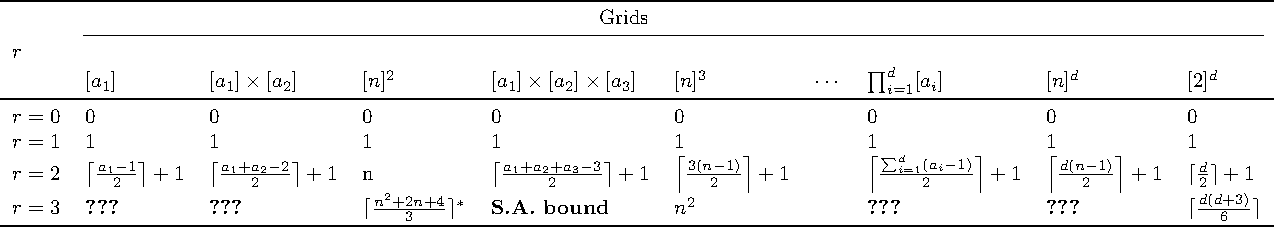
\includegraphics[width=\textwidth,origin=c]{tables/1/known_bounds.pdf}
\caption{A summary of known bootstrap percolation results for grids and the torus, $r \in \{0,1,2,3,d\}$.}
\label{tab:known_bounds}
\end{table} 

We end this introduction with the presentation of a delightful question about the cardinality of $2$-neighbor percolating sets on the two-dimensional lattice. The interested reader in encouraged to find a solution on their own; however, a proof of the result is presented at the beginning of the following section.
\begin{question}
Let $(n,n)$ represent the $n \times n$ lattice, given by $G = P_n \times P_n$. What is $m(n,n,2)$?
\end{question}

\section{Minimum percolating sets and bounds}

\subsection{Foundations}

Let us build some intuition for the behavior of percolating sets on the two-dimensional lattice. Figure \ref{fig:5x5x1} illustrates the percolation time-steps for an arbitrary initial infection on the graph $G=P_5 \times P_5$, where $r=2$. (In general, we shall refer to the $d$-dimensional lattice with sides $a_1, \dots, a_d$ as the $d$-tuple $(a_1, \dots, a_d)$. The standard notation is $\prod_{i=1}^d a_i$.) 

\begin{figure}[]
\centering
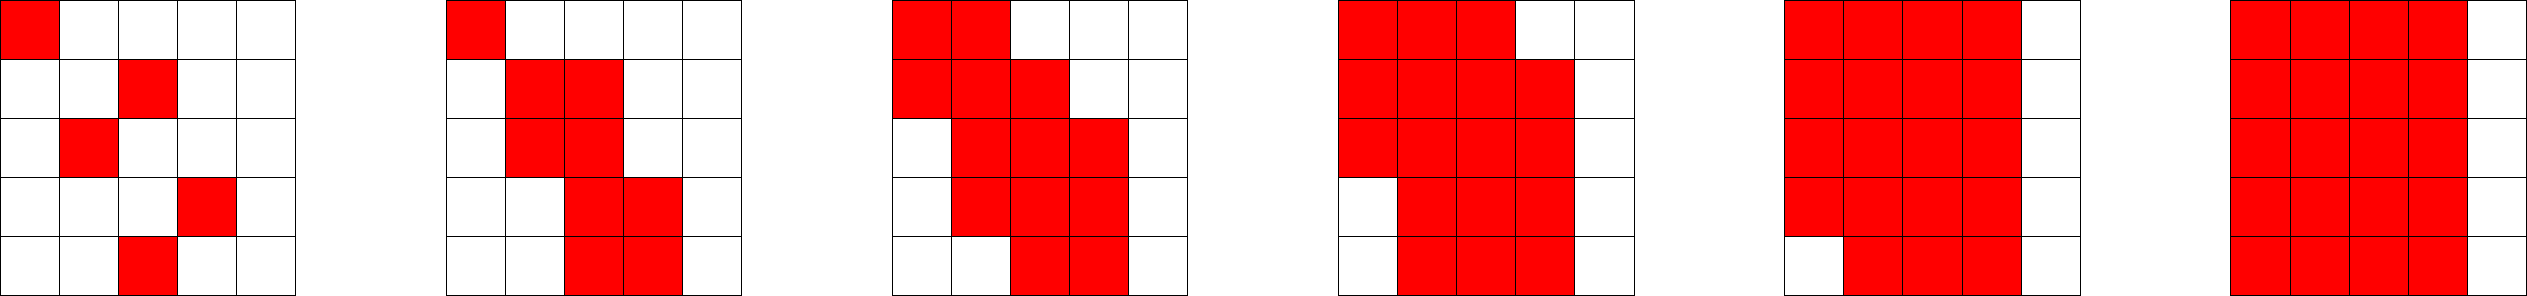
\includegraphics[width=\textwidth]{figures/1/5x5x1.pdf}
\caption{Percolation time-steps for an arbitrary initial infection on the $5 \times 5$ lattice, $r=2$.}
\label{fig:5x5x1}
\end{figure} 

Note that this configuration fails to infect the entire grid; that is, the initial infection is not lethal. Heuristically, this appears to be a consequence of the fact that infected cells are unable to access the healthy cells in the rightmost column. We might, therefore, hypothesize that an initial infection must somehow ``span" the entire lattice. A potential ``spanning" construction is illustrated in figure \ref{fig:5x5x1_improved}. Observe that at each time-step, the infection spreads out laterally from the initial diagonal. It is a simple exercise to verify that this construction is lethal on all $(n,n)$ grids for $r=2$. We also note that a similar construction is lethal on all $(n,m)$ grids for $r=2$ (figure \ref{fig:8x4x1}).

\begin{figure}[]
\centering
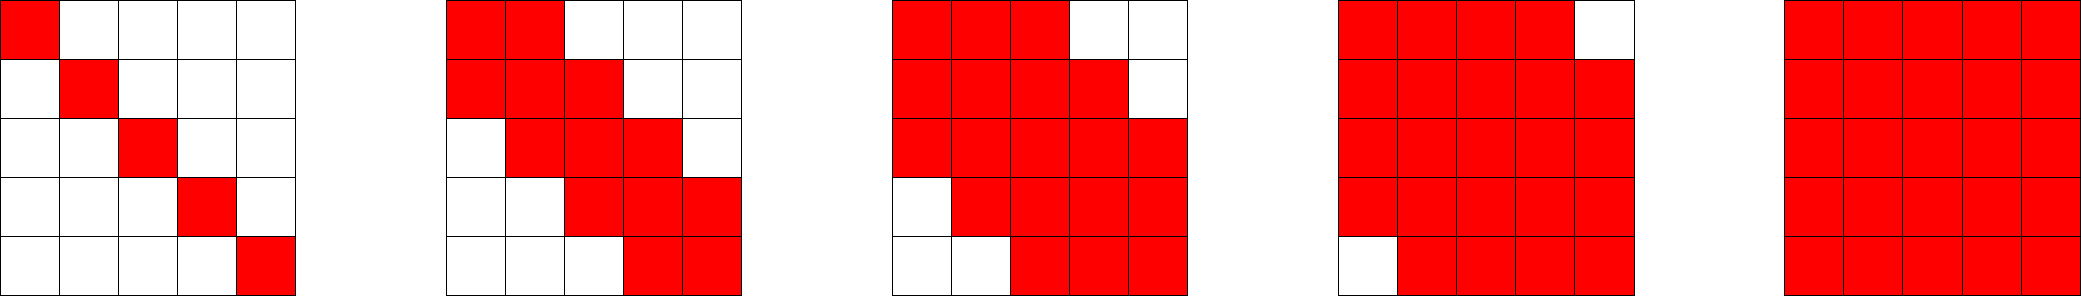
\includegraphics[width=\textwidth]{figures/1/5x5x1_improved.pdf}
\caption{Percolation time-steps for a ``spanning" initial infection on the $5 \times 5$ lattice, $r=2$.}
\label{fig:5x5x1_improved}
\end{figure} 

\begin{figure}[]
\centering
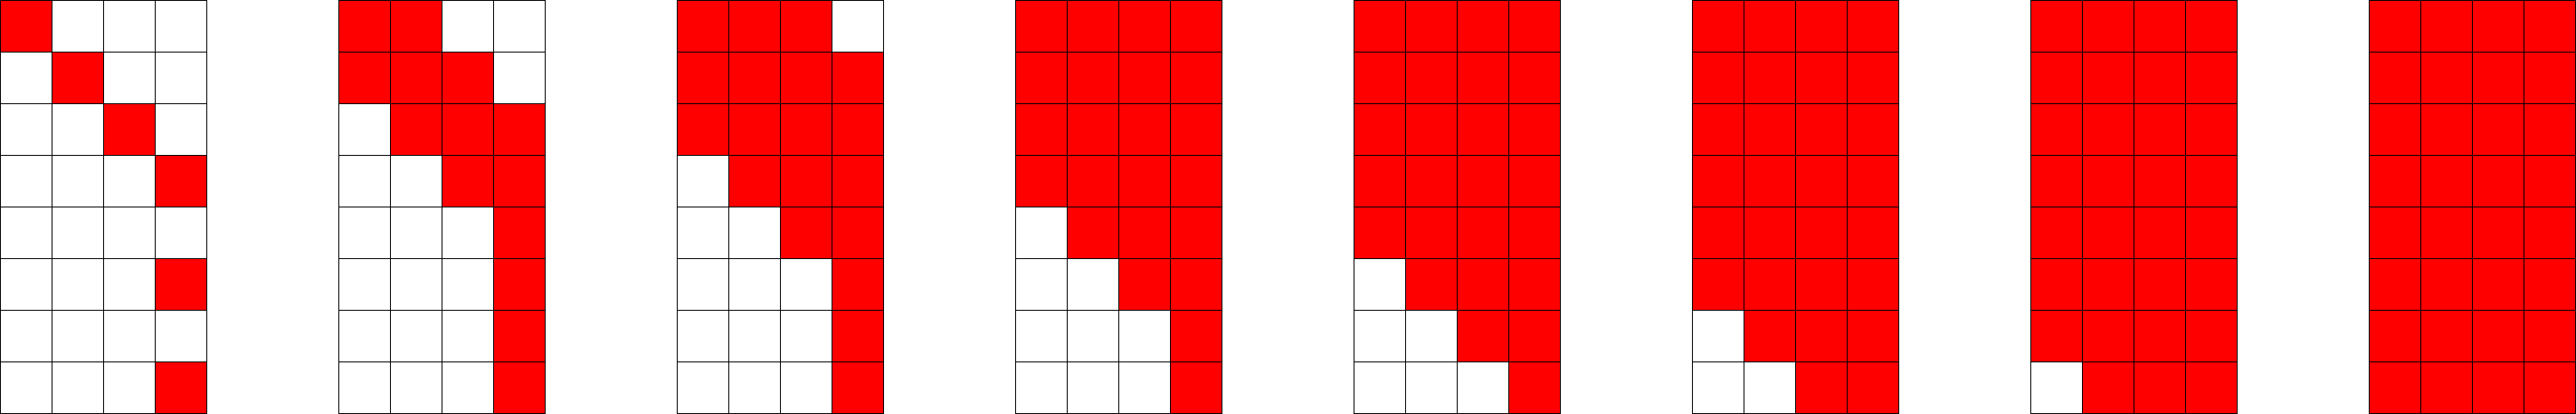
\includegraphics[width=\textwidth]{figures/1/8x4x1.pdf}
\caption{A lethal infection on the $8 \times 4$ lattice, $r=2$.}
\label{fig:8x4x1}
\end{figure} 

The $(n,n)$ construction can be generalized to any dimension. Specifically, we have:

\begin{prop}
\label{prop:nxn_lower_bound}
For all $n,d \geq 1$, 
$$m([n]^d, d) \leq n^{d-1}.$$
\end{prop}
This result has been known since at least Pete \cite{pete:1997}, although the particular constructions are difficult to render in general. The following proof (appearing in \cite{przykucki:2019}, but known in bootstrap percolation ``folklore" for much longer) elegantly shows that this bound is tight.

\begin{thm}
\label{thm:tight_perimeter}
For all $n,d \geq 1$, 
$$m([n]^d, d) = n^{d-1}.$$
\end{thm}

\begin{proof}
The upper bound follows from proposition \ref{prop:nxn_lower_bound}. The lower bound is given by a generalization of the famous ``perimeter argument". Suppose $d=2$ and consider an embedding of $G=[n]^d$ in the $n\times n$ grid. Let $A_0 \subseteq V(G)$ be a set of initially infected cells. We claim that the total perimeter of all infected regions in $G$ is monotonically decreasing as a function of the time-step $t$. Consider an arbitrary healthy cell $c$. In order for $c$ to become infected, at least two of its edges must abut infected cells. However, this implies that (upon infection of $c$) these edges are absorbed within the newly expanded infected region, thereby reducing the perimeter of infection by two. As $c$ contains at most two un-absorbed edges, the perimeter of infection cannot increase. 

Since a lethal set will infect the entire grid, and therefore have a final perimeter of infection of $4n$, it follows that the perimeter of infection of $A_0$ must be at least $4n$, and so $m([n]^2, 2) \geq n.$

The same argument generalizes nicely to higher dimensions. Simply observe that for a given hypercube cell to become infected, it must donate at least $d$ of its $2d$ hyperplane faces to the infected region, thereby at most maintaining the current $(d-1)$-perimeter of infection.
\end{proof}

We note that the perimeter argument extends directly to rectangular grids; however, the problem of obtaining tight constructions, should they exist, is largely unsolved and will be the main focus of this thesis. The following proposition, which we refer to informally as the \emph{surface area bound} or \emph{S.A. bound}, provides a lower bound on the size of lethal sets for $d$-dimensional rectangular grids where $r=d$.

\begin{prop}
\label{prop:SA_bound}
For $d \geq 1$ and $a_1, \dots, a_d \geq 1$,
$$m(a_1, \dots, a_d, d) \leq \frac{\sum_{i=1}^d \prod_{j \neq i} a_j}{d}.$$
\end{prop}

\begin{proof}
Observe that the expression
$$\frac{\sum_{i=1}^d \prod_{j \neq i} a_j}{d}$$
is precisely the high-dimensional perimeter of the grid graph $(a_1, \dots, a_d)$. The bound follows from the perimeter argument in theorem \ref{thm:tight_perimeter}. 
\end{proof}

In \{some chapter of this thesis\}, we will prove that this bound is tight in the case where $d=3$ and $d_1,d_2,d_3 \geq 8$. We fully expect that this bound can be incrementally diminished; however, we feel that such small improvements do not at this time justify the effort required to obtain additional constructions. 

In the remainder of this section, we shall present a number of additional bootstrap percolation results for different classes of grid graphs.

\subsection{Additional results}

Recall from the previous section that $m(n,n,2) = n$, where the tight construction for the lower bound is given by a diagonal infection expanding laterally outwards. In a paper by Balogh and Bollobas \cite{balogh:2006}, this result is generalized to all $d$-dimensional hypercubes $(a_1, \dots, a_d)$, $a_i \geq 1$. 

\begin{thm}
For $d \geq 1$ and $a_1, \dots, a_d \geq 1$, 
$$m(a_1, \dots, a_d, 2) = \ceil*{\frac{\sum_{i=1}^d (a_i-1)}{2}}+1.$$
\end{thm}

\begin{proof}
\end{proof}

As suggested by table \ref{tab:known_bounds}, general results become quite sparse for $r \notin \{2,d\}$. A nice result from Morrison and Noel resolves the question of $r=3$ for hypercubes $P_2^d$ of dimension $d \geq 3$. 

\begin{thm}
For $d \geq 3$ and $a_1 = \dots = a_d = 2$, 
$$m(a_1, \dots, a_d, 3) = \ceil*{\frac{d(d+3)}{6}}.$$
\end{thm}

\begin{proof}
\end{proof}

However, the issue of determining $m(a_1, \dots, a_d, r)$ is largely unresolved. Furthermore, good lower bounds for $r \neq d$ are conspicuously absent. 
\end{comment}
% ^^^ ONE GIANT COMMENT ^^^

